\documentclass{standalone}
\usepackage{tikz}

\usetikzlibrary{mindmap}

\begin{document}
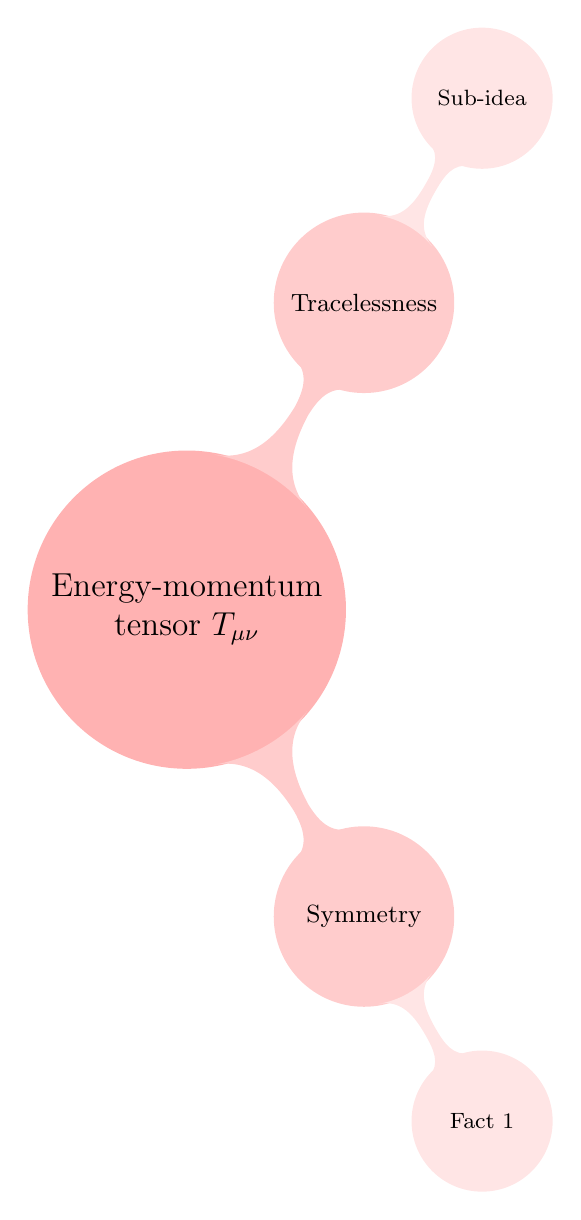
\begin{tikzpicture}[
        mindmap,
        concept color = red!30,
        every node/.style = {concept},
        grow cyclic,
        level 1/.append style = {
                concept color = red!20,
                level distance = 4.5cm,
                sibling angle = 120
            },
        level 2/.append style = {
                concept color = red!10,
                level distance = 3cm,
                sibling angle = 45
            }
    ]

    \node  {Energy-momentum tensor $T_{\mu\nu}$}
    child {node {Symmetry}
            child {node {Fact 1}}
        }
    child {node {Tracelessness}
            child {node {Sub-idea}}
        };

\end{tikzpicture}
\end{document}